%Anfoderungsanalyse

%%%%%%%%%%%%%%%%%%%%%%%%
\chapter{Analyse}
\label{sec:Anforderungsanalyse}
%%%%%%%%%%%%%%%%%%%%
Das Konzept der modularen Anlagen eröffnet neue Möglichkeiten, bringt aber auch neue Herausforderungen. Durch die Flexibilität ist es denkbar, dass Module öfter ausgetauscht werden. Welche Informationen für den Auswahlprozess benötigt werden, wird im folgenden analysiert.

\section{Informationsbedarf}
Der Informationsbedarf orientiert sich maßgeblich an den Aufgaben und dem Nutzer. \todo{weiter ausführen}

\subsection{Modulare Anlage}
Der Lebenszyklus einer modulare Anlage wird in unterschiedliche Phasen eingeteilt. Sie besteht aus Planung, Errichtung, Betrieb und Demontage. \cite{Obst2013} Besonderer Augenmerk in dieser Arbeit liegt auf dem Potential der Flexibilität. So kann die modulare Anlage beispielsweise bei Wartungsarbeiten an einem Modul mit einem alternativen Modul weiter betrieben werden.

Probleme können jedoch nicht nur beim Austausch von Modulen entstehen. Es ist auch denkbar, dass ein Service zurück meldet, das ein Fehler vorliegt. Nun müsste die Ursache gefunden werden. Welche Probleme beim Betrieb der modularen Anlage auftreten können ist in Abschnitt \ref{Probleme-modulare-Anlage} näher beschrieben.

Um diese Probleme lösen zu können muss unter anderem klar sein, welche Informationen zur Verfügung stehen. Für den Austausch von Informationen zwischen Prozessführungsebene (PFE) und Modul wird das Modul Type Package (MTP) verwendet. Da der Modulhersteller entscheiden kann, welche Informationen zur Verfügung gestellt werden, unterscheidet sich der konkrete Inhalt des MTP von Modul zu Modul. Es soll hier nicht auf den konkreten Aufbau des MTPs eingegangen werden.

\subsubsection*{Informationsaustausch mittels MTP}
Das Modul stellt eine Reihe an Informationen zur Verfügung, die durch das Modul Type Package (MTP) beschrieben sind. Im MTP sind unter anderem das HMI und die Services hinterlegt. \todo{Zitat fehlt}

Für einen eindeutigen Austausch von Informationen sind Schnittstellen definiert. Jede Schnittstellendefinition besteht aus einem Erklärungstext und den spezifischen Informationsvariablen. Da für jede Schnittstelle andere Informationen übertragen werden, sind hier nur allgemeine relevante Aspekte gelistet. So können Einheiten, Maximal- und Minimalwerte oder Prozesswerte übermittelt werden.
\begin{itemize}
\item \textbf{TagName:} Name der repräsentierten Information. 
\item \textbf{TagDescription:} Beschreibung der repräsentierten Information, z.B. Innere Temperatur des Reaktors.
\item \textbf{ScaleSettings:} Das Modul teilt der PFE die möglichen Anzeigegrenzen mit.
\item \textbf{UnitSettings:} Übermittelt die Einheit des übertragenen Werts.
\item \textbf{ValueLimitation:} Das Modul gibt die Sollwertgrenzen für bestimmt Parameter vor.
\item \textbf{Feedback Monitoring:} Gibt die Rückmeldung an die PFE, dass eine Fehlfunktion vorliegt.
\item \textbf{Limit Monitoring:} Mittels der Limit Variablen können Werte für Toleranz-, Warnungs- und Alarmgrenzen festgelegt werden. Das Modul überwacht die Variablen und signalisiert eine Grenzwertüberschreitung.
\end{itemize}

\subsubsection*{Services}
Wie bereits in Abschnitt \ref{2:Modulare-Anlagen} beschrieben, werden Module durch Dienste gesteuert. Jeder Dienst kann 16 verschiedene Zustände annehmen und teilt den aktuellen Zustand der PFE mit. Die PFE kann die Zustandsübergänge Reset, Pause, Resume, Unhold, Stop, Abort und Restart anfordern. Bei kontinuierlichen Fahrweisen können zusätzlich Start und Complete angefordert werden. Des Weiteren wird der Zustandsübergang State Change (SC) durch den vorgelagerten Zustand ausgelöst. \todo{Bild einfügen} Die aktuell verfügbaren Zustandswechsel meldet das Modul zurück.

Dienste haben verschiedene Betriebsarten. Sie werden in Offline, Manual, Automatic External und Automatic Internal eingeteilt. Zudem gehört zu jedem Dienst eine Liste mit dem verwendetem Anlagenequipment. Diese Information könnte für eine Eingrenzung des Problembereichs verwendet werden.
%Wenn sich der Dienst nicht in Offline befindet, werden automatisch alle zum Dienst gehörigen Aktoren in Automatic überführt.
%\begin{itemize}
%\item \textbf{Offline:} Dienst ist nicht betriebsbereit und die Aktoren des Dienstes können in Manual überführt werden.
%\item \textbf{Manual:} Der Dienst wird vom Bediener über die PFE oder ein lokales Panel bedient.
%\item \textbf{Automatic External:} Die Zustandsübergänge werden durch die PFE gesteuert.
%\item \textbf{Automatic Internal:} Die Zustandsübergänge werden modulintern ausgelöst.
%\end{itemize}

Sollen Dienste näher spezifiziert werden, ist eine Verwendung von Parametern möglich. Es wird zwischen Konfigurationsparameter, Fahrweisenparametern, Prozesswerten und Reportwerten unterschieden. \todo{Zitat}
\begin{itemize}
\item \textbf{Konfigurationsparameter:} Werden für grundlegende Einstellung verwendet. Ein Ändern ist nur möglich, wenn der Dienst offline ist. Es können beispielsweise ...
\item \textbf{Fahrweisenparameter:} Sind rezeptrelevant, werden vom Dienst beim Starten und Neustart überprüft und bei Zulässigkeit übernommen. Es wird an die PFE rückgemeldet, ob der Parameter übernommen werden konnte. Beispielhafte Parameter sind Sollwerte, wie Temperatur- oder Durchflussvorgaben und Reglerparameter, wie Verstärkung und Nachhaltezeit.
\item \textbf{Prozesswerte:} \todo{ergänzen}
\item \textbf{Reportwerte:} Zur Nachweis- und Dokumentationspflicht werden die Werte in den Zuständen Completed, Aborted und Stopped gespeichert.
\end{itemize}

\subsubsection*{Probleme in modularen Anlagen}
\label{Probleme-modulare-Anlage}
Da die modularen Anlagen mit Diensten gesteuert werden, ändert sich auch die Art an Problemen, die entstehen und die vom Modulbetreiber behoben werden können. Durch die Dienste wird nur noch ein Problembereich angezeigt. Meldet ein Dienst zurück, dass er nicht erfolgreich durchgeführt werden kann so ist noch nicht eindeutig, wo das Problem liegt. Durch die Anzeige von dazugehörigem Equipment und möglichen Serviceabhängigkeiten kann der Problembereich eingegrenzt werden. Bei Betrieb der modularen Anlage im P2O-Lab der TU Dresden treten derzeit die häufigsten Fehler auf, wenn entsprechende Zuläufe nicht geöffnet werden \todo{belegen}. So meldet aktuell das Reaktormodul nicht zurück, wenn vergessen wurde die Druckluft anzustellen. Dem Betreiber fällt nur auf, dass das Modul nicht so arbeitet, wie es soll. Wurde beim Temperiermodul vergessen den Zulauf für das Wasser zur Kühlung zu öffnen, so meldet sich dieses erst nach ca. zwei Minuten zurück, dass es zu warm wird.

Neben den Problemen, die sich relativ einfach auf herkömmliche Anlage übertragen lassen, können im Zuge der Flexibilität ganz Neue entstehen. Die Option nicht nur Parameter anzupassen sondern auch Module auszutauschen, eröffnet neue Möglichkeiten und stellt den Modulbetreiber vor neue Herausforderungen. Müller und Urbas \cite{} \todo{Zitat} haben diesen Gedanken bereits angestoßen. Aus diesem Grund ist es interessant zu begutachten, welche weiteren Faktoren bei einem Modulaustausch relevant werden können.

\subsection{Informationen nach Aufgabenbereich}
Neben den Informationen, die ein Modul zur Verfügung stellt und die bei Behebung einer Störung behilflich sein können, gibt es eine Reihe von weiteren interessanten Aspekten. Weitet man den Problembereich von einer reinen Instandhaltung auf Bereiche wie die Wirtschaftlichkeit aus, so werden ganz andere Informationen benötigt. Welche Funktionen auf welcher Ebene in einem Unternehmen automatisiert werden können und somit auch sinnvoll durch ein Assistenzsystem unterstützbar sind ist in \cite{Lauber1999} beschrieben. Hier ist auch der zeitliche Aspekt mit aufgeführt. Eine entsprechende Übersicht findet sich in Tabelle \ref{tab:Ebenen-Unternehmen}.
\begin{table}[htbp]
\centering
\caption{Ebenen in einem Unternehmen bei Führung technischer Prozesse}
\label{tab:Ebenen-Unternehmen}
\begin{tabular}{|p{0.2 \textwidth}|p{0.33 \textwidth}|p{0.33 \textwidth}|}
\hline
\textbf{Ebenen eines Unternehmens} & \textbf{zeitliche Anforderungen} & \textbf{Automatisierungs-funktionen} \\
\hline
Unternehmens-führung & Entscheidungen wirken sich langfristig aus (nach Monaten oder Jahren) & Kostenanalysen, statistische Auswertungen \\
\hline
Produktions-planung und Betriebsleitung & Änderungen werden nach Tagen, Wochen oder Monaten sichtbar & Betriebsablaufplanung, Kapazitätsoptimierung, Auswertung der Prozessergebnisse \\
\hline
Leitung technische Prozesse & Eingriffe wirken sich nach Stunden oder Minuten aus & Prozessüberwachung, An- und Abfahrten, Störungsbehandlung, Prozessführung, Prozesssicherung \\
\hline
Prozessgrößen & Auswirkungen sind nach Sekunden, Millisekunden oder gar Mikrosekunden sichtbar & Messen, Steuern, Stellen, Regeln, Verriegelungen, Not-Bedienen von Prozessgrößen, Abschalten, Schutz \\
\hline
\end{tabular}
\end{table}

Auf der Unternehmensführungsebene sind beispielsweise folgende Kosten relevant \todo{eventuell löschen, da doppelt} \cite{Kunstler2014}:
\begin{itemize}
\item Logistikkosten
\item Personalkosten
\item Verpackungskosten
\item Kosten für Reklamationen und Retouren
\item Kosten aufgrund fehlender Prozesssynchronisation
\end{itemize}
Folgende Kennzahlen sind für die Produktions- und Betriebsleitebene interessant \cite{Kunstler2014}:
\begin{itemize}
\item \textbf{Kennzahlen der Beschaffung:} Lieferzeiten, Preistrends nach Warengruppen
\item \textbf{Kennzahlen der Produktion:} Auslastung der Geschäftsbereiche, Durchlaufzeiten, Rüstzeiten
\item \textbf{Kennzahlen der Finanzprozesse:} Produktivität- und Wirtschaftlichkeitskennzahlen
\end{itemize}

\subsection{Informationsbedarf der Operator}
\label{3:Informationsbedarf-Operator}
Stützt man sich bei der Ermittlung des Informationsbedarfs auf die individuellen Fähigkeiten und das vorhandene Wissen so ist eine entsprechende Analyse relativ komplex. Insbesondere, wenn der Problemlöseprozess einen Lerneffekt haben soll. In der Literatur ist dies als Assistance Dilemma bezeichnet. Wenn der Lerneffekt möglichst groß sein soll wird Information über die Problemlösung und die Lösungsschritte zunächst zurück gehalten. Informationen werden interaktiv hinzugefügt, wenn sie benötigt werden. Die größte Herausforderung ist dabei die Kriterien festzulegen, wann Informationen gegeben und wann sie zurück gehalten werden\cite{Koedinger2007}.  Richey und Nokes-Malach \cite{Richey2013} empfiehlt eine geringe Bereitstellung an hilfreichen Erklärungen bei Problemlöseaktivitäten, solange andere Ressourcen für den Lernprozess zur Verfügung stehen. Da diese Arbeit den Fokus auf eine geeignete Informationsaufbereitung legt, wird an dieser Stelle nicht weiter darauf eingegangen, wie der Lernerfolg des Menschen ideal unterstützt werden kann. Die Literatur \cite{Miller2005, Sauer2018} hebt hervor, dass Operator ein mittleres Level an Automatisierung bevorzugen. Auf diesem Level werden beim komplexen Problemlösen die meisten Varianten generiert. Bei keiner Unterstützung übersieht der Operator möglicherweise wichtige Aspekte. Bei einer hohen Automatisierung denkt der Operator nicht mehr über Alternativen nach und bestätigt den Vorschlag nur noch. \cite{Miller2005} Im Kontext des Modulaustausch könnte das System verschiedene Vorschläge liefern, die durch Vorschläge des Menschen ergänzt werden können.

In Abschnitt \ref{2:Unterscheidung-Probleme} ist bereits beschrieben, dass komplexe Probleme auf das Wesentliche reduziert werden müssen und häufig Informationsbeschaffung gefordert ist. In dieser Arbeit soll die Informationsbeschaffung unterstützt und die Übersichtlichkeit der Information zur Reduktion der Komplexität gewährt werden.

Welche Informationen sind nun für den Modulbetreiber relevant, wenn ein Modul ausgetauscht werden muss?

Der sicherlich wichtigste Punkt ist die Kompatibilität. Passen die Anschlüsse zu den anderen Modulen der Anlage? Kann das Rezept weiterhin, wie konfiguriert gefahren werden oder sind Anpassungen notwendig? Um dies einschätzen zu können sind weitreichende Informationen über das Modul und die aktuelle Anlage notwendig. Diese umfassen
\begin{itemize}
\item \textbf{die Abmaße:} Passt das Modul von der Größe an die gleiche Stelle, wie das andere Modul?
\item \textbf{die Schnittstellen:} Ist das Modul mit den Schnittstellen der anderen Module kompatibel?
\item \textbf{das Rezept:} Welche Stellen im Rezept werden beeinflusst, wenn das Modul getauscht werden muss?
\item \textbf{die Services:} Welche Serviceabhängigkeiten bestehen zwischen dem Rest der Anlage und dem zu ersetzenden Modul?
\item \textbf{die Parameter:} Können die Parameter bei einem Austausch beibehalten werden oder müssen Anpassungen vorgenommen werden? Wenn Anpassungen vorgenommen werden müssen, welche Auswirkungen hat das auf den Prozess?
\end{itemize}

Ein Modulaustausch hat nicht nur auf der rein technischen Seite einen Einfluss. Ein Unternehmen muss noch viele weitere Faktoren berücksichtigen, um sich bei Alternativen für eine entscheiden zu können. Die Kriterien für die Auswahl werden durch die Ziele des Unternehmens bestimmt. Zur Unterstützung der Zielerreichung ist eine Verwendung von Kennzahlen möglich. Mit den Kennzahlen kann der aktuelle Zustand ermittelt und überwacht werden. Dabei muss auch festgelegt werden, welche Entscheidungsrelevanz die Kennzahl hat.  Bezogen auf den Modulaustausch könnten der Aufwand einer Rezeptänderung oder die Auswirkungen auf die Produktqualität relevant sein. Mit Sicht auf die Produktionsprozesse identifiziert Gottmann \cite{Gottmann2016} eine ganze Reihe von Faktoren, welche die Ziele beeinflussen können (siehe Bild \ref{pic:Produktionsprozesse-Zielgroessen} \citep[50]{Gottmann2016}).
\begin{figure}[htb]
\centering
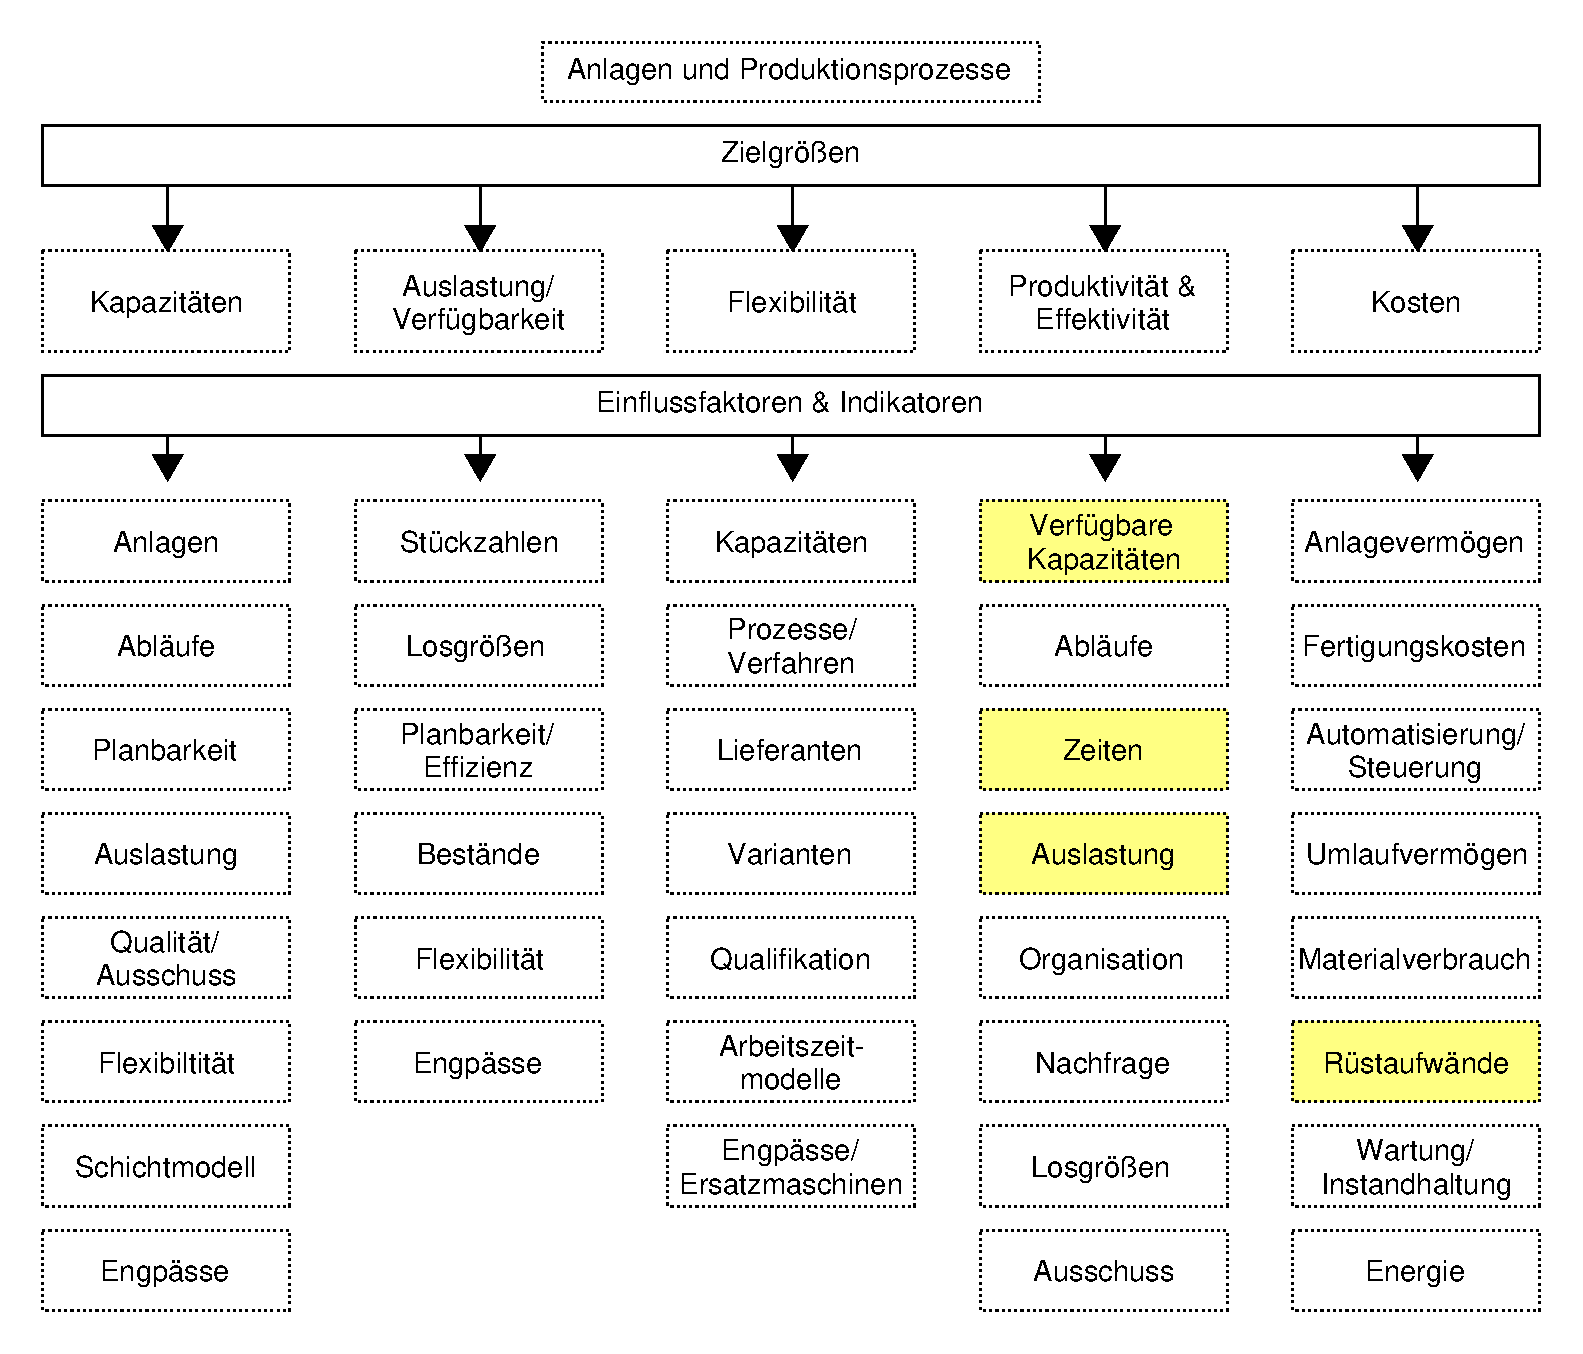
\includegraphics[scale=0.5]{DA_files/Bilder/Analyse/Produktionsprozesse-Zielgroessen.pdf}
\caption{Produktionsprozess: Zielgrößen und Einflussfaktoren}
\label{pic:Produktionsprozesse-Zielgroessen}
\end{figure}

In dieser Arbeiten werden nur einige wenige Einflussfaktoren berücksichtigt. Zum einen ist nicht für jedes Unternehmen jede Zielgröße und somit auch nicht jeder Einflussfaktor relevant. Zum anderen ist beispielsweise die Flexibilität durch die modulare Anlage bereits weitestgehend gewährleistet. In dieser Arbeit wird der Fokus auf die Produktivität \& Effektivität und die Kosten gelegt. Die Produktivität beschreibt, wie viel der verfügbaren Arbeitszeit zur Produktion verwendet wird. Steht aufgrund vieler Störungen in der Anlage die Produktion still, so ist die Produktivität gering. Bei einer hohen Effektivität werden die verfügbaren Ressourcen ideal genutzt. Dies kann beispielsweise die Zeit sein, die eine Reparatur in Anspruch nimmt. Die entstehenden Kosten sind für die Wirtschaftlichkeit der Produktion verantwortlich. \cite{Gottmann2016} Im Kontext des Modulaustausch sind vor allem die Anschaffungs- und Betriebskosten relevant. Folgende Einflussfaktoren sollen im weiteren Verlauf der Arbeit berücksichtigt werden:
\begin{itemize}
\item \textbf{Zeiten:} Wie viel Stillstandzeit verursacht der Modulaustausch?
\item \textbf{Auslastung:} Besteht die Möglichkeit vor zu produzieren?
\item \textbf{Rüstaufwände:} Was muss alles im Rezept verändert werden? Welche Zeit nimmt das in Anspruch und welche Kosten verursacht das?
\item \textbf{Wartung:} Wie häufig muss das neue Modul gewartet werden?
\item \textbf{Energie:} Wie hoch ist der Energieverbrauch des Moduls? Welche Kosten verursacht dies beim Betrieb?
\end{itemize}

\section{Informationsanpassung}
Die Individualisierung von Software bietet die Möglichkeit eine Vielzahl von Nutzer und Aufgaben zu unterstützen. Individualisierung dient der Modifizierung von Interaktion und Informationsdarstellung, um unter anderem den Fähigkeiten und Bedürfnissen jedes Benutzers gerecht zu werden. Ebenso ist auch die Anpassung an das zu lösende Problem nicht zu unterschätzen. Je nach Zielstellung müssen andere Informationen hervor gehoben werden.

\subsection{Individualisierung für den Menschen}
Soll jeder Nutzer des Assistenzsystemes individuell anhand seiner kognitiven Leistung unterstützt werden, so ist herauszufinden, ob der Mensch aktuell mit der Aufgabe über- oder unterfordert ist. Eine Möglichkeit ist die Art und Weise der Interaktion auszuwerten und entsprechende Anpassungen vorzunehmen. Wie bereits in Abschnitt \ref{2:Adaptive-Systeme} beschrieben, sind dabei viele Einflussfaktoren zu berücksichtigen. Eine Auswertung dieser sprengt leider den Rahmen der Arbeit.
\todo{aufführen, welche Individualisierung für den Menschen vorgenommen wird}

\subsection{Anpassung an die Aufgabe}
\label{3:Anpassung-Aufgabe}
Wie schon in Abschnitt \ref{2:Unterscheidung-Probleme} beschrieben, lassen sich Probleme anhand verschiedener Aspekte unterscheiden. So ist zum Beispiel der Zeitdruck ein wichtiger Aspekt. Bei zeitkritischen Problemen muss möglichst schnell eine gute Lösung gefunden werden. Ist das Problem nicht zeitkritisch so können in Ruhe alle zur Verfügung stehenden Informationen in den Problemlöseprozess mit einbezogen werden. So kann bei einem zeitkritischen Problem ein höherer Automatisierungsgrad gefordert sein. Um dennoch dem Menschen seine Kompetenzen nicht abzusprechen, ist es möglich bei Problemen, die eher langfristig sind und die eine höhere kognitive Aktivität erfordern, eine geringere Autonomiestufe anzuwenden. Dadurch kann der Mensch sich Wissen über den Prozess aneignen und seine Kompetenzen ausbauen.

Angenommen der Nutzer hat viel Zeit sich mit dem Problem zu beschäftigen, so müssen sich die bereitgestellten Informationen auch am Probleminhalt orientieren. Der Austausch eines Moduls bedarf einer Übersicht der Kompatibilität mit der bestehenden Anlage und dem Rezept. Entsteht ein Problem aufgrund eines fehlgeschlagenen Services, so ist das zugehörige Equipment und die eingestellten Parameter relevant. Durch die Aufbereitung dieser Informationen und deren Abhängigkeiten kann schrittweise die Ursache gefunden werden.

Ein ebenfalls wichtiger Aspekt, der schon in Abschnitt \ref{3:Informationsbedarf-Operator} thematisiert wurde, ist die Zielsetzung des Unternehmens. Diese kann sehr unterschiedlich sein, was sich maßgeblich auf die Informationsbereitstellung auswirkt. Ist beispielsweise der Energieverbrauch besonders relevant, so sollten diese Informationen über die Module hervor gehoben werden. In einem anderen Kontext kann aufgrund von Personalmangel der Rüstaufwand eine höhere Priorität bekommen. 

\section{Interaktionsmechaniken}
Im Kontext dieser Arbeit wird das Problemlösen betrachtet. Problemlösen heißt in diesem Fall aus mehreren Alternativen die geeignetste für das Erreichen des festgelegten Ziels auszuwählen. In Abschnitt \ref{2:Assistenzsysteme} sind verschiedene Interaktionsmechaniken beschrieben. Um diese geeignet bewerten zu können ist zunächst eine Begutachtung des Arbeitsumfelds und der Aufgaben notwendig.

Da sich das Problemlösen im Rahmen dieser Arbeit nicht auf das Beheben von Störungen bezieht, kann angenommen werden, dass die Hände nicht für andere Aufgaben frei sein müssen. Zudem ist eine geeignete Darstellung von Zusammenhängen notwendig, welches eine entsprechende Displaygröße voraussetzt. Diese Zusammenhänge müssen durch den Menschen entsprechend interpretiert werden, damit dieser mit dem System interagieren kann. Es muss dazu die Möglichkeit gegeben sein selbst Vorschläge für die Lösung des Problems zu liefern. Das setzt vielfältige Eingabemöglichkeiten voraus.

Daraus abgeleitet wird für die Umsetzung des Assistenzsystem ein Tablet verwendet. Diese ist groß genug, um alle notwendigen Informationen anzuzeigen. Es ist flexibel genug, wenn für den Problemlöseprozess Informationen benötigt werden, die nur durch Begutachtung der Anlage erlangt werden können. Zudem bietet die Kamera die Möglichkeit Augumented Reality zu verwenden oder das Mikrofon die Möglichkeit Spracheingaben zu tätigen.

\section{Use Case}
\todo{vielleicht woanders hin schieben}
Steht ein Modul aufgrund von umfangreichen Wartungsarbeiten nicht zur Verfügung so müssen Alternativen gefunden werden. Das übergeordnete Ziel ist die Aufrechterhaltung der Produktion. Das System könnte nun mögliche Alternativen vorschlagen, die von den Abmaßen und Schnittstellen verwendet werden können.
\begin{itemize}
\item \textbf{Modul A:} Ist identisch mit dem Modul, das gewartet wird und kann beim Modulhersteller geliehen werden. Dieser fordert eine Leihgebühr. Eine Anpassung im Rezept muss nicht vorgenommen werden.
\item \textbf{Modul B:} Wurde ursprünglich verwendet und aufgrund eines hohen Energieverbrauchs ersetzt.
\end{itemize}
Angenommen es existiert noch ein Modul C, welches vom System nicht in Erwägung gezogen wird, da es nicht die geforderten Schnittstellen zur Verfügung stellt. Diese kann manuell vom Menschen vorgeschlagen werden, da dieser weiß, dass mit entsprechenden Adaptern eine Integration in die Anlage möglich ist.

Nun stehen drei Module zur Verfügung, aus denen eins ausgewählt werden muss. In Tabelle x sind die Vor- und Nachteile der einzelnen Module aufgelistet. Diese Vor- und Nachteile müssen nun vom Operator abgewägt werden. Dabei steht ihm das Assistenzsystem zur Seite. Diese könnte mit folgenden Informationen Unterstützung leisten:
\begin{itemize}
\item Zeigt Bereiche im Rezept an, die angepasst werden müssen.
\item Berechnet die laufenden Kosten, die entstehen, wenn die Wartung des ursprünglichen Moduls länger dauert
\item ....
\end{itemize}

\begin{table}[htbp]
\centering
\begin{tabular}{|p{0.14 \textwidth}|p{0.23 \textwidth}|p{0.23 \textwidth}|p{0.23 \textwidth}|}
\hline
\textbf{Modul} & Modul A & Modul B & Modul C \\
\hline
\textbf{Vorteile} & keine Anpassungen im Rezept nötig & Kostengünstig; Gewissheit, dass es funktioniert & geringer Energieverbrauch \\
\hline
\textbf{Nachteile} & hohe Leihgebühr & hoher Energieverbrauch, einige Anpassungen im Rezept notwendig & viele Anpassungen im Rezept notwendig \\
\hline
\end{tabular}
\caption{x}
\label{tab:}
\end{table}

\section{Anforderungen an das Assistenzsystem}

\subsection{Funktionale Anforderungen}

\subsubsection*{Unterstützung der Problemidentifikation}
\begin{itemize}
\item[PI 1] Der Nutzer soll durch die Problemlösung begleitet werden können, indem...
	\begin{itemize}
	\item[PI 1.1] ...er das Problem beschreibt.
		\begin{itemize}
		\item[PI 1.1.1] z.B.: Das Temperiermodul muss gewartet und der Prozess dabei aufrecht gehalten werden.
		\end{itemize}
	\end{itemize}
	\begin{itemize}
	\item [PI 1.2] ...er das Ziel definieren kann.
		\begin{itemize}
		\item[PI 1.2.1] Festlegung des Zeitdrucks: z.B. Wartung findet in 2 Tagen statt
		\item[PI 1.2.2] Festlegung der Zielgröße: z.B. Prozess muss mit geringem Kostenverlust weiter laufen
		\end{itemize}
	\item[PI 1.3] ...ihm alle Informationen über die aktuelle Situation zur Verfügung stehen.
		\begin{itemize}
		\item[PI 1.3.1] Aktuelles Rezept
		\item[PI 1.3.2] Aktueller Aufbau der Anlage
		\item[PI 1.3.3] Übersicht über die KPIs
		\end{itemize}
	\end{itemize}
\end{itemize}

\subsubsection*{Unterstützung bei der Problemlösung}
\begin{itemize}
\item[PL 1] Das Assistenzsystem soll mögliche Lösungen vorschlagen können.
	\begin{itemize}
	\item[PL 1.1] Diese sollen sich an den festgelegten Zielen orientieren.
	\item[PL 1.2] Die Auswirkungen auf die Anlage/ den Prozess müssen dargestellt werden.
	\end{itemize}
\item[PL 2] Der Nutzer soll mögliche Lösungen vorschlagen können.
\item[PL 3] Die Lösungen sollen bewertbar sein.
\end{itemize}

\subsubsection*{Kluster von Problemen}
\begin{itemize}
\item[KP 1] Es sollen mehrere Probleme gleichzeitig bearbeitet werden können.
\item[KP 2] Die Probleme sollen sich sortieren lassen.
\item[KP 3] Die Probleme sollen mit Merkmalen versehen werden können.
	\begin{itemize}
	\item[KP 3.1] Zeit: Problem ist zeitkritisch und muss schnell gelöst werden oder es ist viel Zeit vorhanden, um über eine mögliche Lösung nachzudenken.
	\item[KP 3.2] Komplexität: Wird die Problemlösung durch viele oder wenige Größen beeinflusst?
	\end{itemize}
\end{itemize}

\subsection{Nichtfunktionale Anforderungen}
\begin{itemize}
\item[NA 1] Die Bedienung soll über ein Tablet realisiert werden.
\end{itemize}
